\documentclass[a4paper]{panl}
\usepackage{cite}
\usepackage{wrapfig}
\usepackage{graphicx}
\usepackage{amssymb}
\usepackage{amsfonts}
\usepackage{amsmath}
\usepackage{longtable}
\usepackage{rotating}
\usepackage{lscape}
\usepackage{epsfig}
\usepackage{multirow}
\originalTeX
%\russianTeX
\begin{document}
% Journal sections (see http://pkp.jinr.ru/index.php/PEPAN_LETTERS/about/editorialPolicies#focusAndScope)
%\issuearea{Physics of Elementary Particles and Atomic Nuclei. Theory}
% or in Russian
\issuearea{ФИЗИКА ЭЛЕМЕНТАРНЫХ ЧАСТИЦ И АТОМНОГО ЯДРА. ТЕОРИЯ}
\title{Анализ химического состава при сканировании транспортных контейнеров гамма-излучением \\ Chemical composition analysis for X-ray transport container scans.}
\maketitle
%\authors{A. Zelenaya$^{~a,}$\footnote{E-mail: zelyenaya.av@phystech.edu}, M. Zelenyi$^{~a,b,}$\footnote{E-mail: mihail.zelenyy@phystech.edu}, A.A.Turinge$^{~a}$,  V.G. Nedorezov$^{~a,}$\footnote{E-mail: vladimir@cpc.inr.ac.ru}}
%\from{$^{a}$\,Institute of Nuclear Research of RAS}
%\vspace{-3mm}
%\from{$^{b}$\,Moscow Institute of Physics and Technology}

\authors{А. В. Зелёная$^{~a,}$\footnote{E-mail: zelyenaya.av@phystech.edu}, М. Е. Зелёный$^{~a,b,}$\footnote{E-mail: mihail.zelenyy@phystech.edu}, А.А.Туринге$^{~a}$,  В.Г. Недорезов$^{~a,}$\footnote{E-mail: vladimir@cpc.inr.ac.ru}}
\from{$^{a}$\,Институт ядерных исследований РАН}
\vspace{-3mm}
\from{$^{b}$\, Московский физико-технический институт}
\begin{abstract}
% Russian translation of the abstract
Для обеспечения национальной безопасности важен контроль перемещения опасных или стратегически важных грузов, таких как взрывчатые вещества, радиоактивные материалы, редкие и драгоценные металлы. Проводить такой контроль можно сканирую содержимое   транспортных контейнеров гамма излучением. В данной работе рассмотрена существующая методика дуальных энергий и предложен альтернативный способ, основанный на измерении энергетического распределения гамма-квантов. Для оценки было проведено моделирование с помощью транспортного кода GEANT4.  Также выполнен эксперимент по измерению энергетического разрешения детектора на основе сцинтиллирующего кристалла BGO и кремневого фотоумножителя. 
\vspace{0.2cm}
It is important for national security to control the movement of dangerous or strategically cargo such as explosives, radioactive materials, rare and precious metals. This control can be provided by scanning transport containers by gamma rays.
In this report the existing technique for scanning (dual energy method) is considered and the alternative method based on measuring the energy distribution of gamma rays is proposed. For estimation perspectives of the proposing method, the  corresponding simulation was conducted by using the GEANT4 toolkit. The example of the algorithm of reconstruction the chemical composition of the scanned object is also considered. In addition the experiment for estimation energy resolution of the detector based on a scintillation crystal BGO and SiPM was carried out.\\
\end{abstract}
\vspace*{6pt}

\noindent
PACS: 02.70.$-$c; 23.20.Nx; 32.90.$+$a

\newpage
\label{sec:intro}
\section*{Введение}
Использование высокоэнергетического гамма-излучения в прикладной томографии уже широко распространено. В этой статье мы рассмотрим возможности улучшения существующего метода как путем модернизации оборудования, так и путем разработки математических алгоритмов, которые более полно используют информацию, содержащуюся в измеренных значениях.
\section*{Метод дуальных энергий}
\begin{figure}[t]
    \begin{center}
        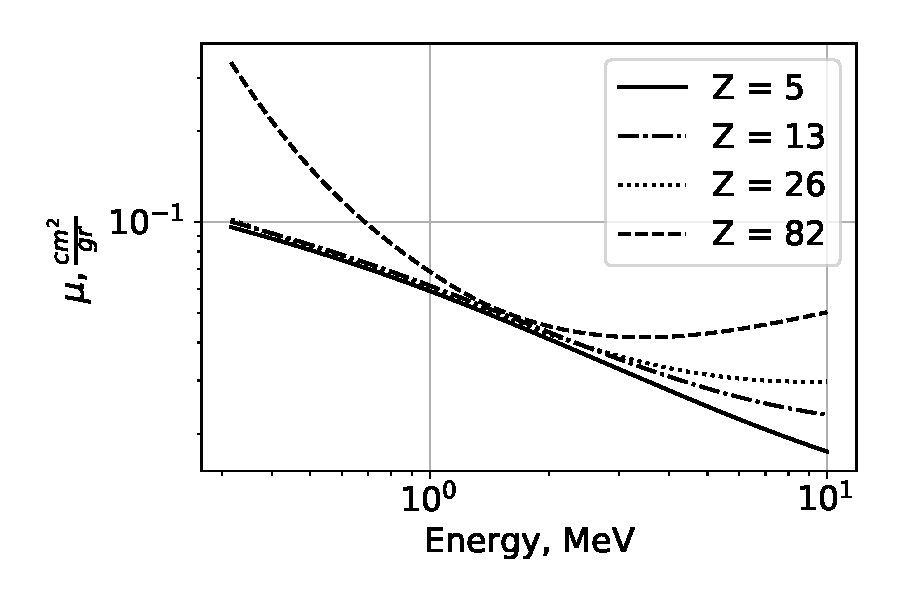
\includegraphics[width=60mm]{figures/Attenuation.pdf} 
        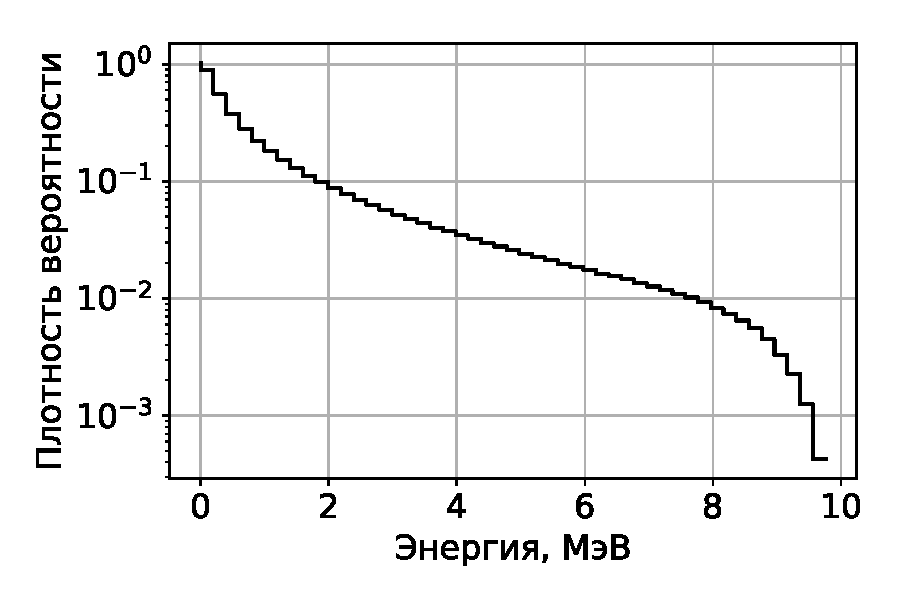
\includegraphics[width=60mm]{figures/Bremsstrahlung.pdf}  
        \vspace{-3mm}
        \caption{а)Массовый коэффициент ослабления для различных материалов б)Спектр тормозного излучения от электрона с энергией 10 МэВ}
    \end{center}
    \labelf{pic:att}
    \vspace{-5mm}
\end{figure}
Рассмотрим, как уменьшается поток гамма-лучей. Коэффициент пропускания описывается следующим уравнением:
\begin{equation}
\label{eq:trans}
T(E_0, t, Z) = \frac{\int \limits_0^{E_0} S(E_0, E) \exp(-\mu(E,Z)\times t)~dE)}{\int \limits_0^{E_0} S(E_0, E)~dE},
\end{equation}
где $T$ -  прозрачность материала для гамма-излучения, $S(E_0, E)$ - функция отклика детектора, $\mu(E,Z)$ - массовый коэффициент ослабления, $t$ -  оптическая толщина материала, $E_0$ - предельная энергия тормозного излучения, $E$ - энергия гамма-излучения, $Z$ - заряд ядра исследуемого материала.
\textbf{Предположим, что как источник гамма-лучей  используется тормозное излучение со спектром как на рисунке ~\ref{pic: att}б и максимальной энергией, зависящей от энергии электронного пучка. Наш коэффициент прозрачности  $T(E_0, t, Z)$ также зависит от среднего массового коэффициента ослабления материала. Рисунок ~\ref{pic: att}а показывает зависимость коэффициента ослабления от энергии для различных материалов. Мы можем выделить три области: начальную, в которой доминирует фотоэлектрический эффект, выделяются только материалы с большим ядерным зарядом; среднее, в котором доминирует комптоновское рассеяние, и материалы не различимы, а область, где основное влияние возникает при производстве электрон-позитронных пар, и материалы достаточно хорошо различимы ~\cite{heitler1984quantum, ALLISON2016186, spirin}. Последняя область может быть использована для метода дуальных энергий ~\cite {spirin}.}

Уравнение~\ref{eq:trans} не позволяет определить материал, если неизвестна оптическая толщина материала. Для решения этой проблемы в методе дуальной энергии предлагается использовать два электронных пучка с различной энергией. Используя прозрачность для двух предельных энергий гамма-лучей $ E ^ {(1)} _0 $ и $ E ^ {(2)} _ 0 $, а затем минимизируя этот функционал:
\begin{equation}
F(z) = \frac{|t(E^{(1)}_0,z) - t(E^{(2)}_0,z)|}{t(E^{(1)}_0,z)} \to min
\end{equation}
становиться возможным исключить неизвестную оптическую толщину и вычислить эффективное зарядовое число для исследуемого материала. Данный метод позволяет отнести сканируемый материал к одной из четырёх групп, разделённых по эффективному зарядовому числу: $Z_{eff} \sim 5$, $Z_{eff} \sim 13$, $Z_{eff} \sim 26$, $Z_{eff} \sim 82$.\\
Однако, метод дуальной энергии имеет некоторые недостатки, среди которых мы выделим два:
    \begin{itemize}
        \item Необходимость в двух пучках различной энергии ведет к усложнению конструкции сканера.
        \item Данный метод будет иметь малую эффективность в случае материала, состоящего из сильно различающихся по заряду элементов.
    \end{itemize}
Поэтому, мы предлагаем альтернативный подход:
    \begin{itemize}
        \item Использовать только один электронный пучок с энергией 10 МэВ.
        \item Измерять не только пространственное, но и энергетическое распределение гамма-квантов 
    \end{itemize}

\section*{Моделирование}
\begin{figure}[t]
    \begin{center}
        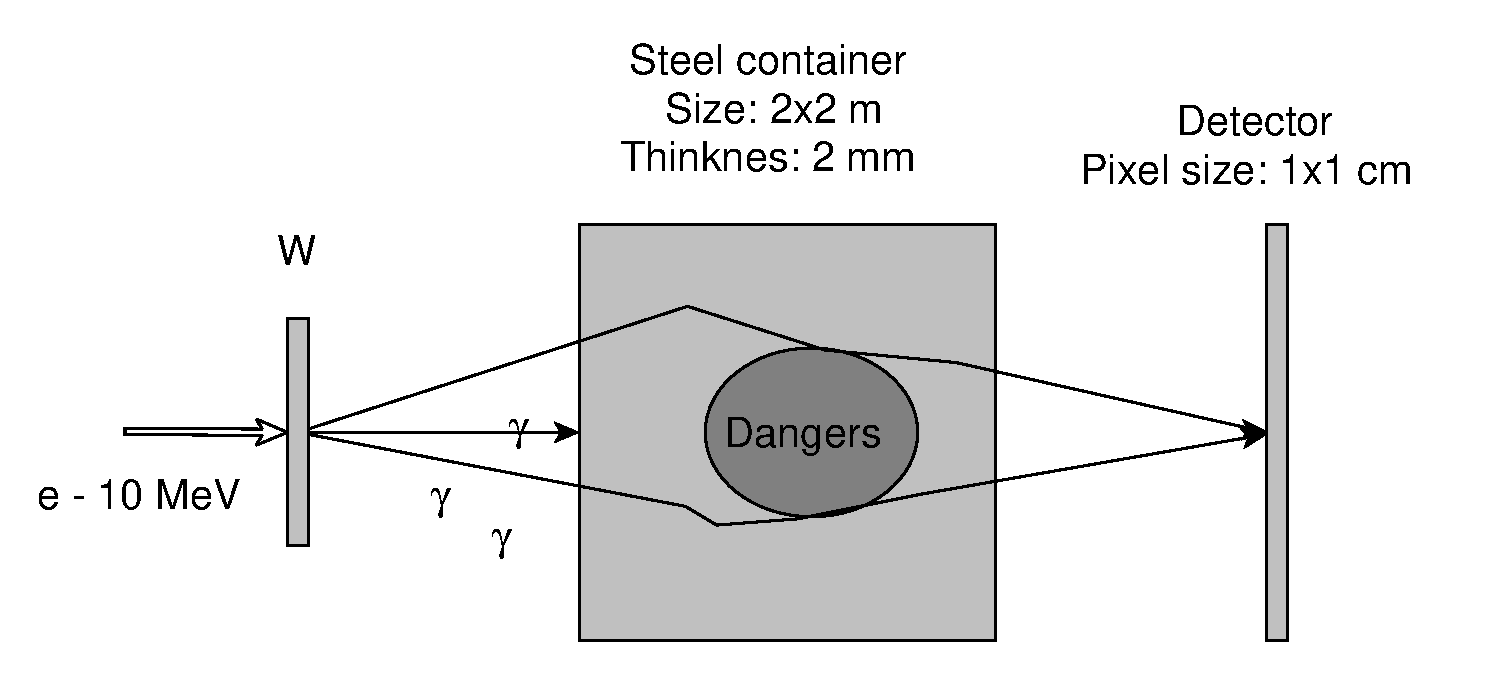
\includegraphics[width=120mm]{figures/yed_schema_1.pdf}
        \vspace{-3mm}
        \caption{Схема симуляции}
    \end{center}
    \labelf{pic:schema1}
    \vspace{-5mm}
\end{figure}
Для оценки мы провели несколько GEANT4~\cite{ALLISON2016186} симуляций, используя схему (рис.~\ref{pic: schema1}): электронный пучок с энергией 10 МэВ сталкивается с вольфрамовым конвертором, создавая тормозное излучение, которое облучает стальной двухметровый контейнер, внутри которого находится сканируемый объект и регистрируется детектором. Расстояние между вольфрамовым конвертором и контейнером составляет два метра, между контейнером и детектором - 10 см. Приведем несколько примеров проведенного моделирования.
\begin{figure}[t]
    \begin{center}
        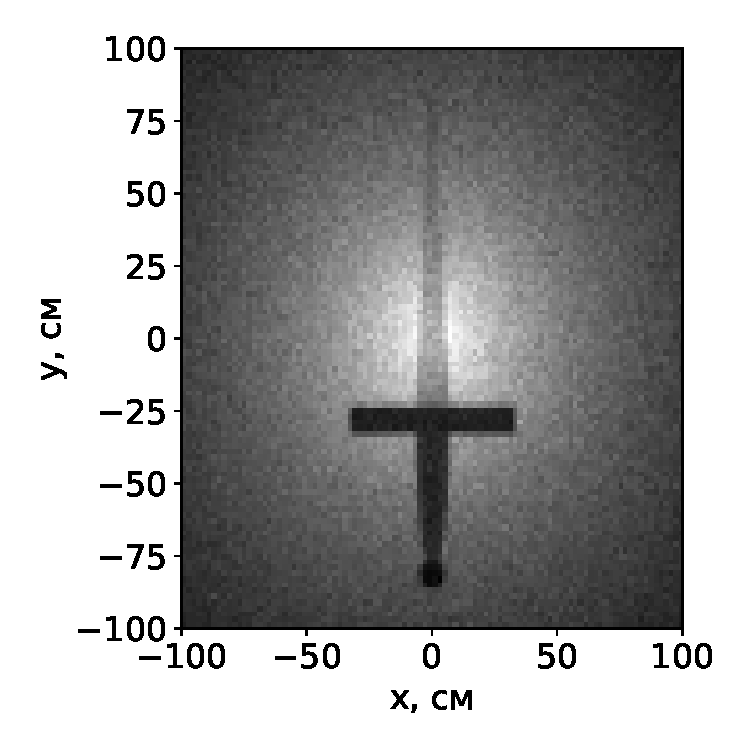
\includegraphics[width=60mm]{figures/Sword.pdf} 
        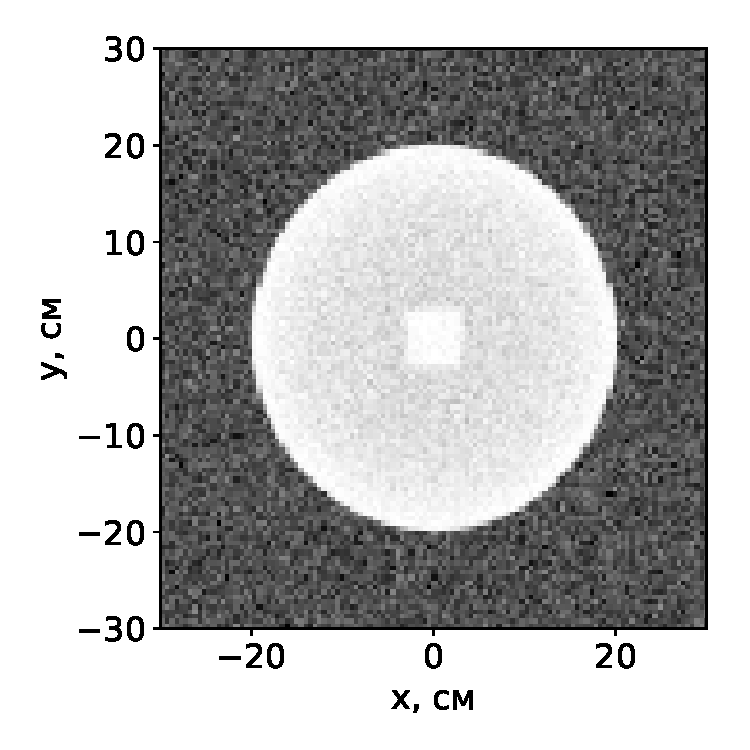
\includegraphics[width=60mm]{figures/UranCube1.pdf}  
        \vspace{-3mm}
        \caption{а)Опасный стальной предмет с неравномерной толщиной б) Кубик урана в свинцовой оболочке}
    \end{center}
    \labelf{pic:sword}
    \vspace{-5mm}
\end{figure}
\begin{figure}[t]
    \begin{center}
        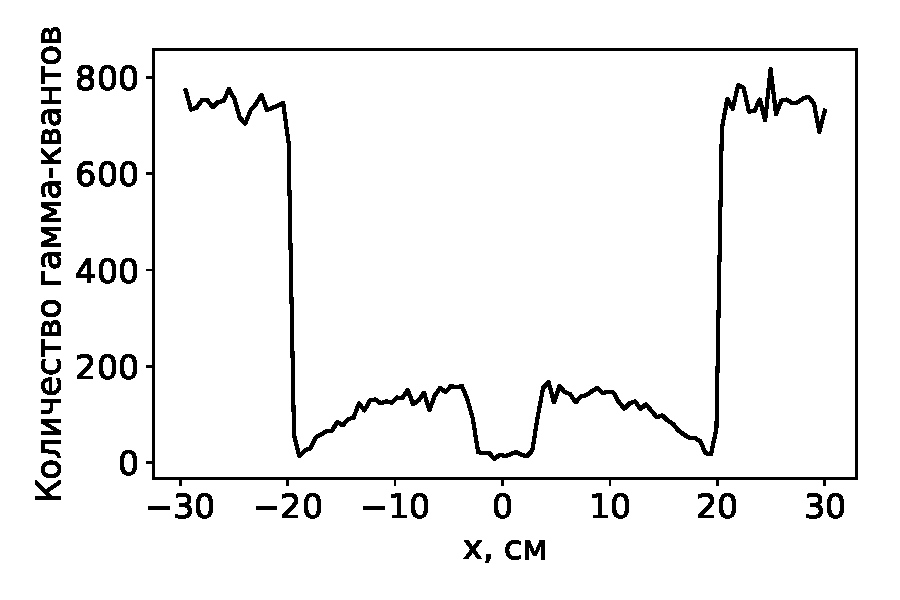
\includegraphics[width=60mm]{figures/UranCube2.pdf} 
        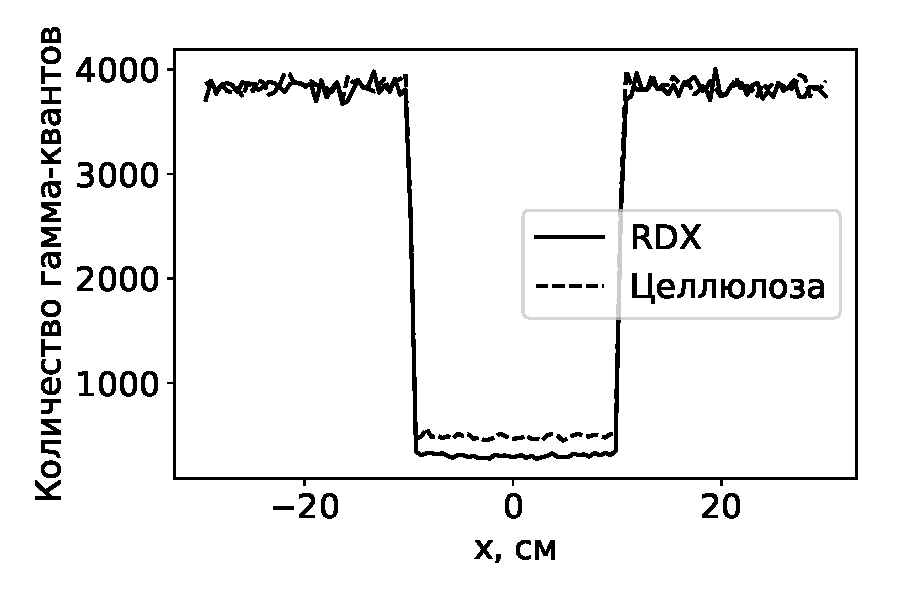
\includegraphics[width=60mm]{figures/Hex.pdf}  
        \vspace{-3mm}
        \caption{а) Кубик урана в свинцовой оболочке б)Сравнение целлюлозы и гексогена}
    \end{center}
    \labelf{pic:hex}
    \vspace{-5mm}
\end{figure}
\begin{figure}[t]
    \begin{center} 
        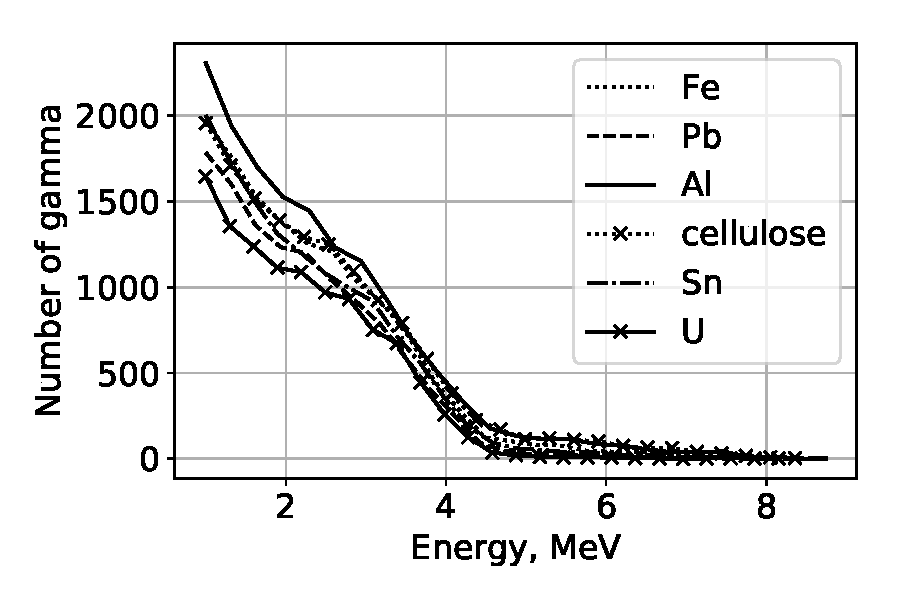
\includegraphics[width=60mm]{figures/diffmat0.pdf} 
        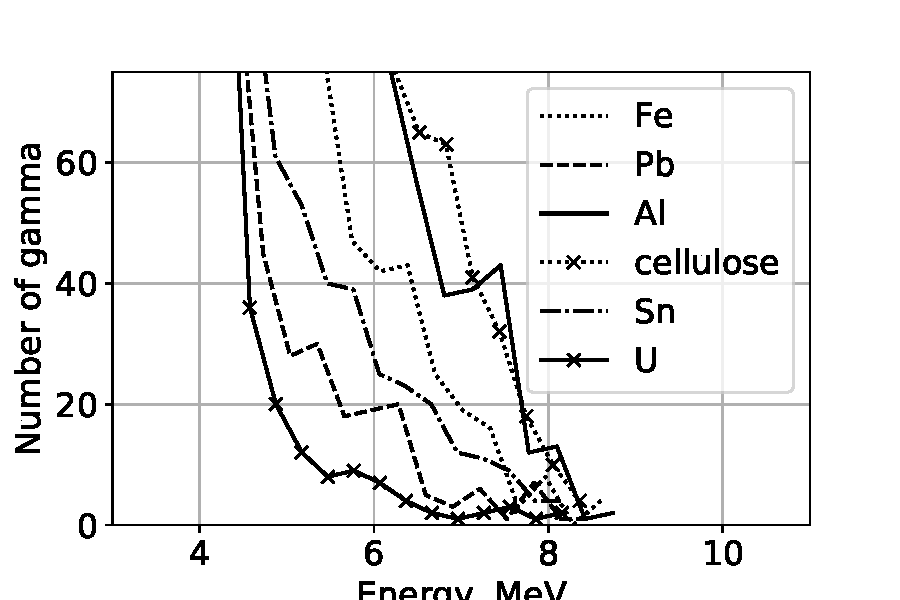
\includegraphics[width=60mm]{figures/diffmat.pdf}  
        \vspace{-3mm}
        \caption{а) Энергетические спектры различных материалов (общий вид)
        б) Энергетические спектры различных материалов (участок с энергией более 4 МэВ)}
    \end{center}
    \labelf{pic:diff0}
    \vspace{-5mm}
\end{figure}
\begin{figure}[t]
    \begin{center}
        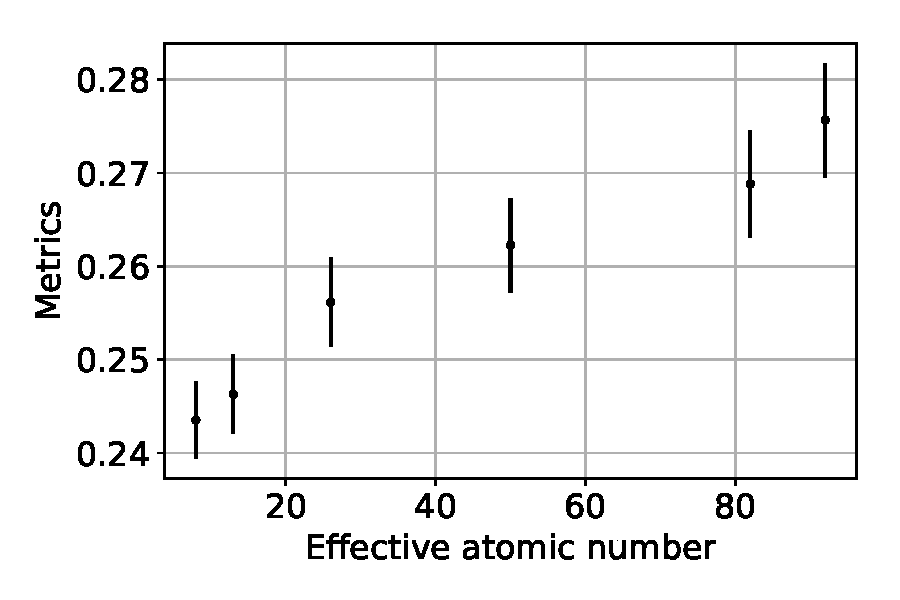
\includegraphics[width=60mm]{figures/diffmat1.pdf} 
        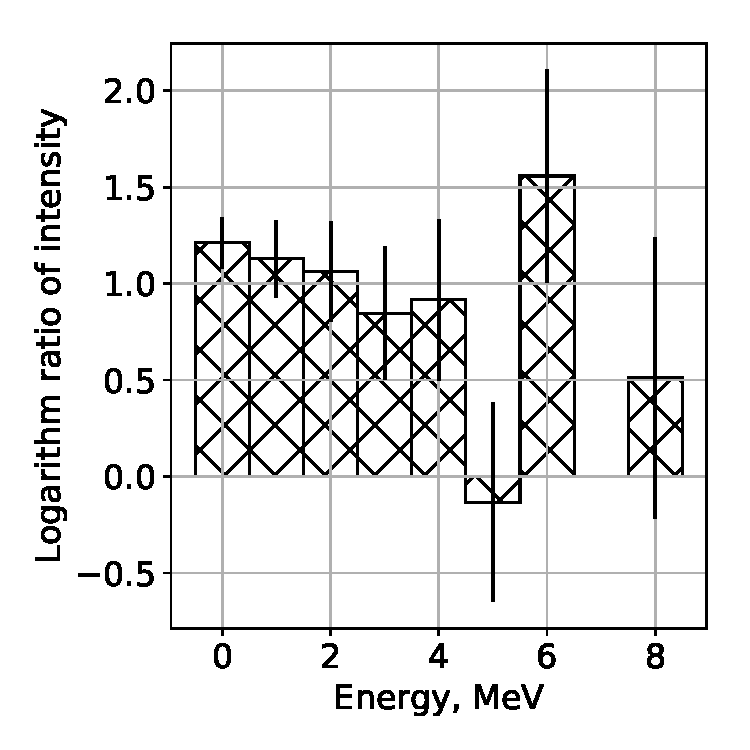
\includegraphics[width=60mm]{figures/Difference.pdf}  
        \vspace{-3mm}
        \caption{а) Зависимость метрики от эффективного зарядового числа материала
 б) Сравнение энергетических спектров из урановых и алюминиевых сфер}
    \end{center}
    \labelf{pic:diff}
    \vspace{-5mm}
\end{figure}
Figure~\ref{pic:sword}a shows an example of a dangerous steel object of non-uniform thickness close to the thickness of the container walls. Figures~\ref{pic:sword}b and~\ref{pic:hex}a show the result of simulation an uranium cube with an edge of 6 centimeters (weight is about 4 kg) placed in a lead sphere with the thickness is 1 cm. As shown by simulation such a cube can be detected with a shell thickness of up to 5 centimeters. Figure~\ref{pic:hex}b demonstrates the difference between two organic materials: safe -- cellulose, and dangerous -- RDX. The difference is significant, which means that it is possible to create algorithms for the searching for organic explosives. The picture~\ref{pic:diff}b shows the result of comparing two energy spectra (the logarithm of the intensity ratio is selected as the metric) from aluminum and uranium sphere of 1 cm in diameter. As we can see, even on such small scales and small (as compared with real beam) intensities it is possible to register differences in the energy spectra.

Also to test the ability for determining the effective charge of the material on the energy spectrum, the following simulation was performed. Six targets were taken from various materials (iron, lead, aluminum, cellulose, tin, uranium), with the same lateral dimension and different longitudinal size. The longitudinal size was chosen in such a way that the total attenuation of the gamma-ray flux would be the same for all materials, and they could not be distinguished only by analysing the spatial spectrum.
The energy spectra of these targets are shown in the figures. As you can see all the spectra are different in the region up to 3 MeV (see the fig.~\ref{pic:diff0}a) and in the region after 4 MeV (see the fig.~\ref{pic:diff0}b). It should be noted that this difference is significant even for small electron beam intensities ($10^8$), which means that in a real electron beam from an accelerator ($10^{15}$) it will be more pronounced. Thus, based on simulations, it is possible to start with a simple criterion: ratio. Such a criterion allows us to distinguish materials by the $Z_{eff}$, and it should be noted that the errors in the figure~\ref{pic:diff} are only statistical and at intensities corresponding to the real electron beam will be negligible. However, this criterion also is not the optimal solution, since when it is used, most of the information about the spectrum is lost. In the next section, we used a simple example to show the potential for creating a 3D gamma-tomography using full spectrum information.
\section*{Восстановление толщин материалов}
\begin{wrapfigure}[9]{r}{0.6\linewidth} 
    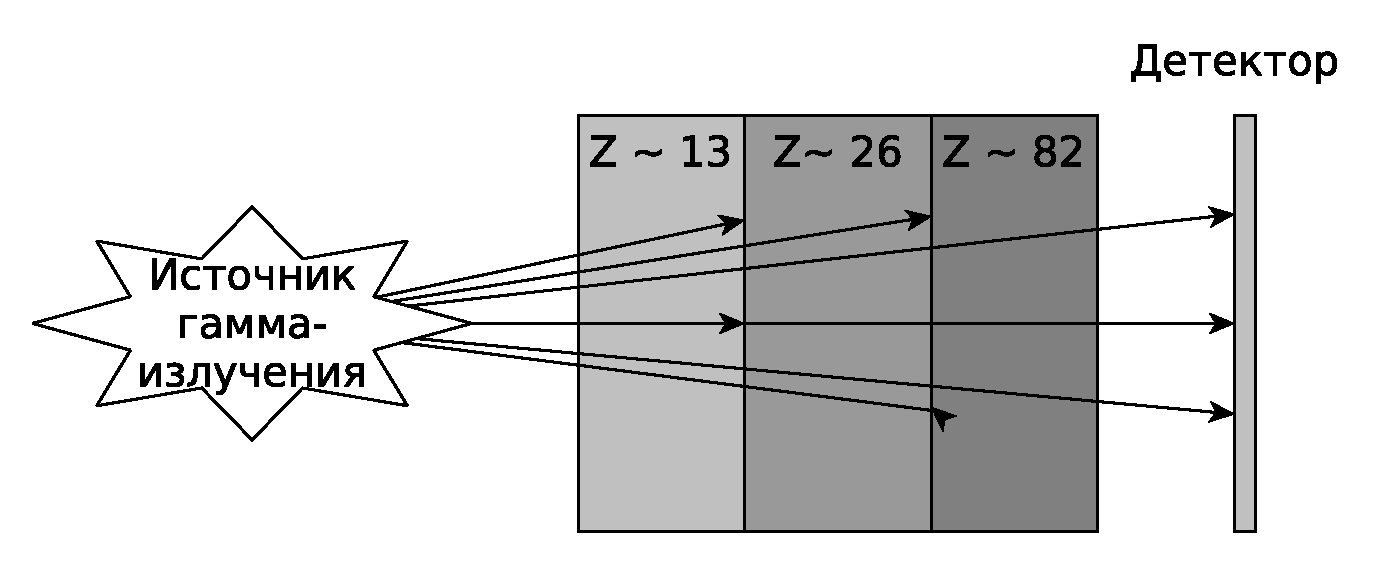
\includegraphics[width=\linewidth]{figures/yed_schema_2.pdf}
    \vspace{-3mm}
    \caption{Восстановление толщин материалов (схема моделирования)}
    \labelf{schema2}
    \vspace{-5mm}
\end{wrapfigure}
Рассмотрим одномерный случай, когда гамма-лучи проходят стопку из нескольких материалов с фиксированной общей толщиной, и нам нужно восстановить толщину отдельных материалов (см. диаграмму~\ref{schema2}). Мы используем простую модель, в которой ослабление потока гамма-излучения задается следующим уравнением
\begin{equation}
\label{eq:gamma}
\frac{N(E)}{N_0(E)} = \exp(-\sum_i \Sigma^{mean}_i(E)x_i),
\end{equation}
где $ x_i $ --- толщина $ i $ -слоя, $ \ Sigma ^ {mean} _i $ --- среднее макроскопическое сечение для группы материалов с близкими зарядовыми числами, $ N, ~ N_0 $ --- количество гамма-квантов. В этом случае мы не учитываем многократное рассеяние и наличие аннигиляционной линии. Мы считаем, что общая толщина известна и для восстановления толщины отдельных слоев мы используем метод наименьших квадратов, т. е. минимизируем такую сумму:
\begin{equation}
\sum_E(\ln \frac{N(E)}{N_0(E)} + \sum_i \Sigma^{mean}_i(E)x_i))^2 \to min
\end{equation}
Приведем пример работы алгоритма. Мы будем считать что энергетическое разрешение составляет величину 10\%. Рассмотрим стопку из трех слоев: алюминиевого, железного и свинцового. Рисунок~\ref{rec:ex}а показывает вклад каждого восстановленного материала в общее ослабление потока гамма-лучей. Таблица~\ref{tab:rec} содержит результаты восстановления для данного примера. Как мы видим из таблицы результат восстановления довольно точный.Чтобы прояснить возможности алгоритма, мы провели несколько численных экспериментов. Мы также как и в примере использовали алюминий, железо и свинец, и взяли около двухсот наборов с разным соотношение толщин слоев, причем суммарная толщина лежала в диапазоне от 30 до 180 сантиметров. Рисунок~\ref{rec:ex}б показывает разброс ошибки восстановления для данных наборов.Как мы можем видеть толщина тяжелых элементов определяется лучше всего - с точность порядка 5\%, а толщина элементов из группы железа хуже всего - величина ошибки достигает 30\%. Однако, мы рассматривали весьма простую модель и возникает вопрос какая от неё польза? В данной модели мы использовали только энергетическое разрешение и по нему смогли провести восстановление послойной структуры объекта. При добавлении пространственного распределение, мы можем провести дополнительно сегментирование в вдоль ещё одно оси и с учетом временной компоненты восстановить трехмерную структуру груза контейнера (3D гамма-томографию). Таким образом наша простая модель показывает, что у нас есть перспектива создания действительно мощной системы для анализа содержимого контейнеров.
\begin{figure}[t]
    \begin{center}
        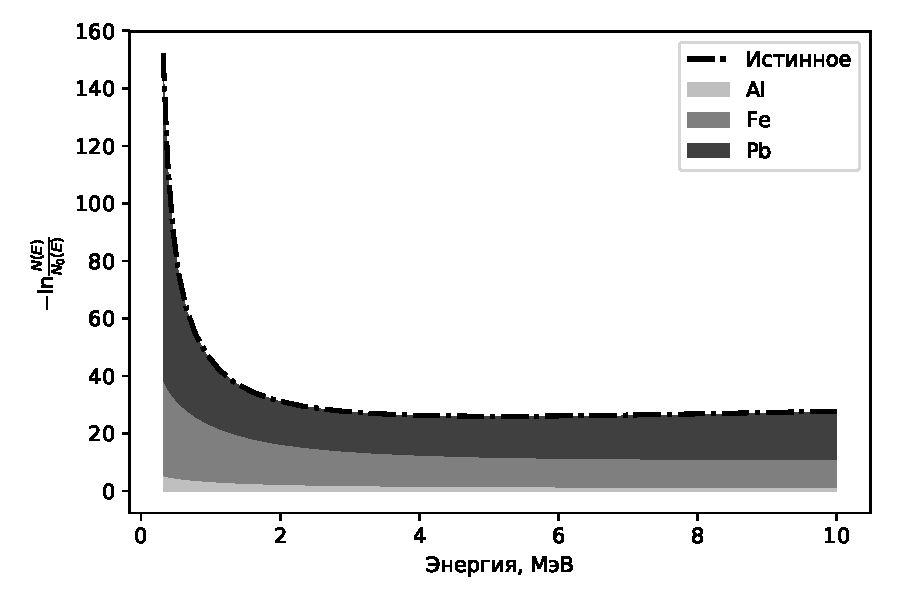
\includegraphics[width=60mm]{figures/reconstruction.pdf} 
        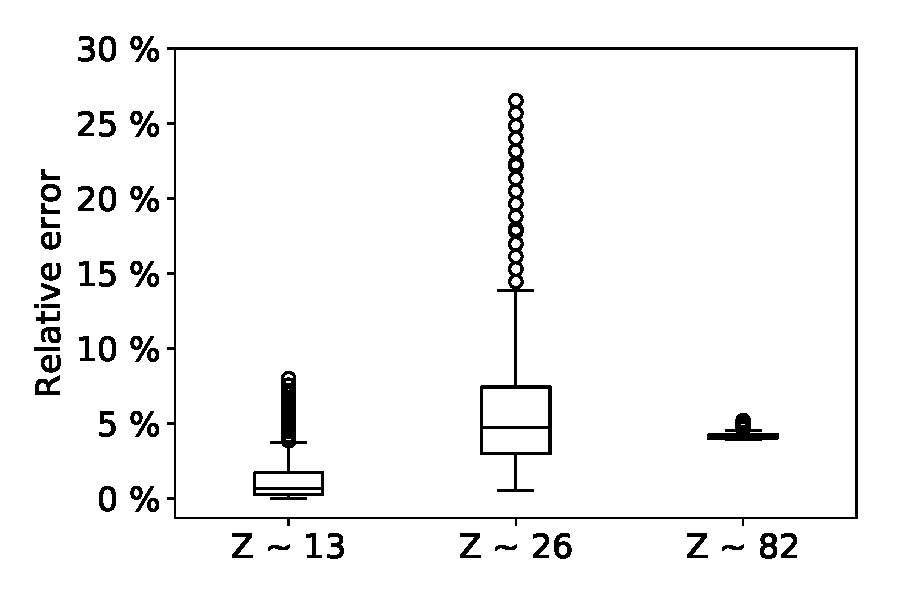
\includegraphics[width=60mm]{figures/relError.pdf}  
        \vspace{-3mm}
        \caption{а) Вклад отдельных слоев в полное ослабление потока б)Распределение ошибок восстановления для различных численных экспериментов}
    \end{center}
    \labelf{rec:ex}
    \vspace{-5mm}
\end{figure}

\begin{table}
    \caption{Пример результата  работы алгоритма восстановления}
    \label{tab:rec}
\begin{center}
        \begin{tabular}[c]{|c|c|c|}
        \hline 
        Материал & Истинная толщина, см & Восстановленная, см \\ 
        \hline 
        Al & 20 & 19.6 \\ 
        \hline 
        Fe & 40 & 41.6 \\ 
        \hline 
        Pb & 30 & 28.7 \\ 
        \hline 
    \end{tabular}
\end{center}
\end{table}

\newpage
\section*{Измерение энергетического разрешения детектора}
%\begin{wrapfigure}[20]{r}{0.5\linewidth} 
%    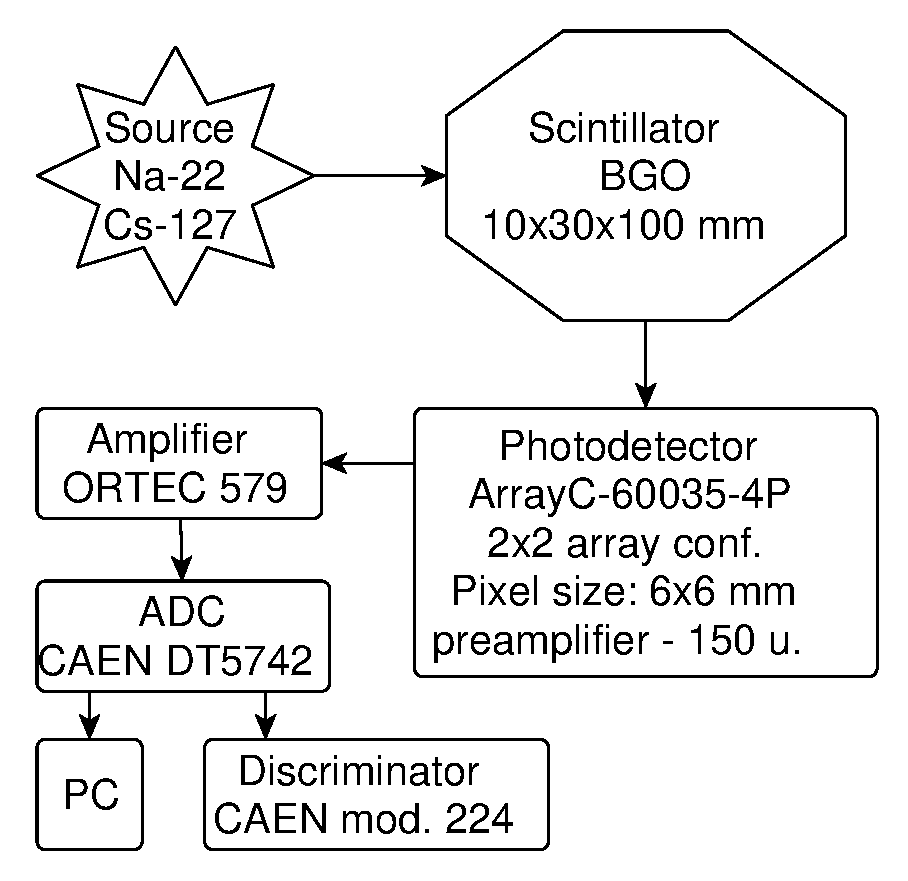
\includegraphics[width=\linewidth]{figures/yed.pdf}  
%    \vspace{-3mm}
%    \caption{Schema of experiment}
%    \labelf{pic:experiment}
%    \vspace{-5mm}
%\end{wrapfigure}
%Вопрос Ивашкины и Губером
В дополнение к моделированию, было измерено энергетическое разрешение энергетического разрешения сцинтилляционного детектора гамма-излучения. В качестве сцинтиллятора использовался кристалл BGO размером 10x30x100 мм ( глубина кристалла подбиралась так что бы обеспечить полное поглощение гамма-квантов до 10 МэВ), для регистрации излучения сцинтиллятора использовался фотодетектор ArrayC-60035-4P. В качестве источников излучения использовались $^{22}Na$ (имеет две линии 0.511 МэВ и 1.275 МэВ) и $^{137}Cs$ (имеет линию 0.662 МэВ). Фотодетектор ArrayC-60035-4P  представляет из себя матрицу из четырёх фотодиодов размером 6x6 мм, оснащенную индивидуальным предусилителем с коэффициентом усиления равным 150.  В процессе работы измерялся суммарный сигнал с двух фотодиодов матрицы. Сигнал c матрицы подавался на усилитель (ORTEC 579) и затем поступал на входной канал АЦП (CAEN DT5742) и на дискриминатор (CAEN mod.224), логический сигнал которого служил триггером в системе. В отсутствие источника шкала АЦП была прокалибрована в абсолютных единицах – числе фотоэлектронов. В таблице~\ref{tab:ex} представлен результат измерения разрешения детектора -  отношения СКО $\sigma_E$ фотопика к его положению $E$. Световыход составляет 140 фотоэлектронов на МэВ, а порог шумов величину порядка 100 КэВ.\\
\begin{table}
    \caption{Измерение энергетического разрешения детектора}
    \label{tab:ex}
    \begin{center} 
        \begin{tabular}[c]{|c|c|c|}
            \hline 
            Источник & Энергия, МэВ & $\frac{\sigma_E}{E}$\\
            \hline 
            $^{22}Na$&0.511 & 19.0 \%  \\ 
            \hline 
            $^{137}Cs$&0.662 & 14.7\%\\ 
            \hline 
            $^{22}Na$& 1.275 & 13\% \\
            \hline 
        \end{tabular} 
    \end{center}
\end{table}


\section*{Выводы}
Результаты:   
    \begin{enumerate}
        \item Измерение  $Z_{eff}$.
        \item Энергетическое разрешение порядка 10 \% позволяет определить толщину отдельного слоя в многослойной структуре с точностью 25\%.
        \item Измерено энергетическое разрешение детектора на основе BGO, полученные результаты близки к характеристикам заявленным производителем ( $FWHM \sim 9\%$ для $^{137}Cs$). В целом полученные результаты говорят о высоких эксплуатационных характеристиках и качестве материала.
    \end{enumerate}
Развитие данной тематике является перспективным направлением деятельности, но требует финансовой поддержки, при наличии которой, становиться возможным разработка программы для проверки содержимого транспортного контейнера заявленному манифесту, и создание программы для гамма-томографии содержимого контейнеров.\\
Данная работа профинансирована в рамках госзадания № 3.3008.2017/ПЧ Министерства Образования и Науки Российской Федерации, и частично выполнена при поддержке гранта РНФ № 16-12-10039.
\bibliographystyle{pepan}
\bibliography{references.bib}

\end{document}
